\subsection{Sparse linear algebra}
Unlike dense linear algebra, computations of sparse problems are irregular.
%
This is mainly due to the matrix storage format.
%
Indeed, to have an efficiently storage, we only store non-zero values of sparse matrices.
%
The non-zero pattern of the matrix is define by the problem we tried to resolve.
%
Some storage formats are optimized for some class of problem, but there is also very generic format.
%
The most generic formats is COO (fig.~\ref{fig:COO}).
%
In COO format, one can store all non-zero values with their 2D coordinates.
%
Another well use format is CSR\footnote{Compress Sparse Row} (fig.~\ref{fig:CSR}) where all non zeros are sorted by row.
%
The row id of a non zero value is then obtain through the array PTR.

\begin{figure}[!ht]
     \begin{center}
        \subfigure[Sparse matrix example]{%
            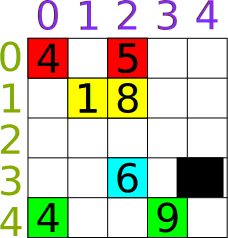
\includegraphics[width=0.25\textwidth]{matrix_format}
        }%
        \subfigure[COO storage]{%
           \label{fig:COO}
           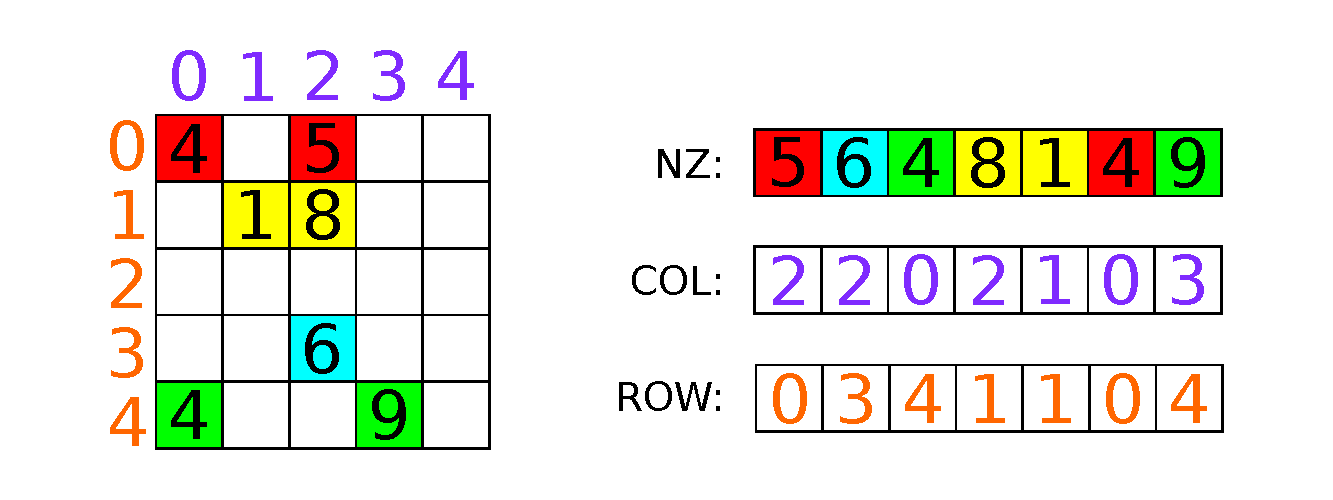
\includegraphics[width=0.35\textwidth]{COO}
        }%
        \subfigure[CSR storage]{%
            \label{fig:CSR}
            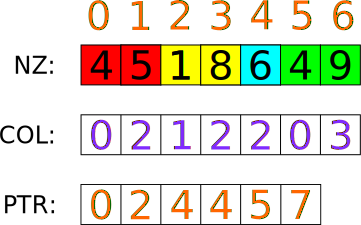
\includegraphics[width=0.35\textwidth]{CSR}
        }%
    \end{center}
    \caption{Comparison between COO and CSR matrix format storage.}
    \label{fig:matrix_storage}
\end{figure}

The choice of the storage format has a lot impact over the performance of an application.
%
With most of format, we will have to do at least two memory access to obtain 2D coordinate of a non zero value whereas in dense algebra it could be calculate from the position in the matrix.
%
A non negligible part of the memory bandwidth is used only for the 2D coordinate.
%
The sparsity and irregularity properties of these matrices also imply to have inefficient memory use in sparse kernel because of bad cache reuse.
%
Most of the optimizations done is dense linear algebra can't be applied to sparse linear algebra because of irregularity in computation and data accesses.
%
But in sparse linear algebra, one can solve much more larger problems than in dense linear algebra.
%
This is because with equivalent matrix dimension, dense linear algebra used much more memory than sparse linear algebra.


Solving sparse linear problems is also different of solving dense linear ones.
%
We cannot use direction inversion of the matrix or gaussian elimination because it will result a quasi-dense matrix, which can't be realizable both in term of memory and in term of computation when the matrix dimension is high.
%
So different methods have been invented to be able to solve these problems, most of them are based on iterative methods.
%
We first start with a solution, then these algorithms reduce iteratively the difference between our approximate solution and the real solution.
%
At the end, we obtain a good approximate solution which is often quite enough to be consider as the solution of the problem.
